% Template for Cogsci submission with R Markdown

% Stuff changed from original Markdown PLOS Template
\documentclass[10pt, letterpaper]{article}

\usepackage{cogsci}
\usepackage{pslatex}
\usepackage{float}
\usepackage{caption}

% amsmath package, useful for mathematical formulas
\usepackage{amsmath}

% amssymb package, useful for mathematical symbols
\usepackage{amssymb}

% hyperref package, useful for hyperlinks
\usepackage{hyperref}

% graphicx package, useful for including eps and pdf graphics
% include graphics with the command \includegraphics
\usepackage{graphicx}

% Sweave(-like)
\usepackage{fancyvrb}
\DefineVerbatimEnvironment{Sinput}{Verbatim}{fontshape=sl}
\DefineVerbatimEnvironment{Soutput}{Verbatim}{}
\DefineVerbatimEnvironment{Scode}{Verbatim}{fontshape=sl}
\newenvironment{Schunk}{}{}
\DefineVerbatimEnvironment{Code}{Verbatim}{}
\DefineVerbatimEnvironment{CodeInput}{Verbatim}{fontshape=sl}
\DefineVerbatimEnvironment{CodeOutput}{Verbatim}{}
\newenvironment{CodeChunk}{}{}

% cite package, to clean up citations in the main text. Do not remove.
\usepackage{apacite}

% KM added 1/4/18 to allow control of blind submission


\usepackage{color}

% Use doublespacing - comment out for single spacing
%\usepackage{setspace}
%\doublespacing


% % Text layout
% \topmargin 0.0cm
% \oddsidemargin 0.5cm
% \evensidemargin 0.5cm
% \textwidth 16cm
% \textheight 21cm

\title{Children's understanding of others' lexical knowledge}

\usepackage{booktabs}
\usepackage{longtable}
\usepackage{array}
\usepackage{multirow}
\usepackage{wrapfig}
\usepackage{float}
\usepackage{colortbl}
\usepackage{pdflscape}
\usepackage{tabu}
\usepackage{threeparttable}
\usepackage{threeparttablex}
\usepackage[normalem]{ulem}
\usepackage{makecell}
\usepackage{xcolor}


\begin{document}

\maketitle

\begin{abstract}
In conversation, if you want to be understood without being overly
informative, you need to figure out what the other person knows, and
what they do not know. For young children to become effective
communicators then, they must learn to infer and update what others are
likely to know. We asked children ages 4-8 (\emph{n} = 62) to make
specific predictions about whether a very young child would know 15
familiar animal words, all typically acquired within a 6-month range.
With minimal information about the target child, children as young as 4
years old inferred that the target child would be more likely to know
easier, earlier-acquired words (e.g., \emph{dog}) and less likely to
know harder, later-acquired words (e.g., \emph{lobster}). These
inferences were increasingly strong across the tested age-range, and
older children also offered {[}more sophisticated explanations for the
child's knowledge{]}. Even preschool-age children make rich inferences
about another agent's lexical knowledge, reflecting robust
metalinguisitc knowledge about when particular words are learned.

\textbf{Keywords:}
communication, metalinguistics, knowledge reasoning, cognitive
development
\end{abstract}

\hypertarget{introduction}{%
\section{Introduction}\label{introduction}}

Imagine visiting the zoo with your friend and their 2-year-old. As you
walk by the peacocks, you hear your friend say, ``Do you see those blue
birds?'' Immediately, you know that your friend is talking to their
child and not you. If they were talking to you, saying ``peacock'' would
be perfectly clear; however, ``blue bird'' might be a better description
for a child who has never seen a peacock before. Even when talking about
the same object, we use different words depending on what we think our
conversational partners know and don't know.

Adults track and adapt to their conversational partners' knowledge with
relative ease. For example, adults reduce the information they give when
re-telling a story to someone who has heard it before, but not when
telling the story to a new partner (Galati \& Brennan, 2010). Adults can
adapt even to partners who are quite different from them, as in the case
of parents and their children. Parents have accurate models of their
children's vocabularies, and use these models in spontaneous
communication, as in the ``blue bird'' example above (Fenson et al.,
2007; Leung, Tunkel, \& Yurovsky, in press; Masur, 1992). Parents'
models of their children's vocabulary are shaped by extensive individual
interactions, but they likely also rely on general metalinguistic
knowledge--for instance, that shorter words are typically simpler than
longer words and thus more likely to be in children's vocabularies.

In a large-scale study, Kuperman, Stadthagen-Gonzalez, \& Brysbaert
(2012) asked adult participants to report the age at which they
understood a given word and obtained judgments for 30,000 English words.
These judgments were then directly compared with data on average age of
acquisition, the typical age that a given word is actually learned
(hereafter referred to as AoA). Adults typically overestimate the
absolute age at which they learned a given word; however, the estimated
order in which words are acquired is intact (Kuperman et al., 2012).
Adults, even adults without children, are able to make graded and
surprisingly accurate relative estimates of when a word was learned.

Can children use this same kind of information to predict whether others
will know words? Pre-school age children are able to infer other
people's knowledge from relatively sparse information, such inferring
knowledgeability based on age or expertise (Jaswal \& Neely, 2009; Lutz
\& Keil, 2002). Further, children ascribe different levels of general
knowledge to infants, preschool children, and adults (Fitneva, 2010;
Taylor, Cartwright, \& Bowden, 1991). By at least age 6, children
understand that there are even some topics where children may know more
than adults, such as toys or children's television (Fitneva, 2010;
VanderBorght \& Jaswal, 2009).

However, reasoning about another person's specific lexical knowledge may
prove difficult for young children as they also show consistent errors
in reasoning about other's knowledge, commonly over-attributing
knowledge (e.g., Gopnik \& Astington, 1988; Taylor, Esbensen, \&
Bennett, 1994). The bias to over-attribute knowledge is particularly
pronounced when the child themselves knows the piece of information
(Birch \& Bloom, 2003; Ghrear et al., 2020).

We ask how children infer another children's lexical knowledge, and
specifically whether they make word-level predicitons in line with
expected AoA. Children at least as young as 5 can make metalinguistic
judgments about their own vocabulary knowledge, reporting the relative
age at which they learned a variety of words (Walley \& Metsala, 1992).
In our study, we introduced 4- to 8-year-old children to a younger
fictional child, and asked them to make judgments about the target
child's knowledge of various familiar words. We find that even
4-year-olds make accurate inferences about the target child's knowledge,
and that older children's responses more closely correlate with adult
judgments of AoA.

\hypertarget{method}{%
\section{Method}\label{method}}

\hypertarget{stimuli}{%
\subsubsection{Stimuli}\label{stimuli}}

Our stimuli consisted of 15 words drawn from a single domain (animal
words), along with corresponding images of each animal. We pulled all
animal images (n = 45) from a normed image set (Rossion \& Pourtois,
2004; recoloring of Snodgrass \& Vanderwart, 1980). To ensure our
stimuli set spanned a range of AoAs, we ranked the animal words from
earliest to latest AoA, using data from Kuperman et al. (2012), and
split the words into five bins. In order to select animal images that
are recognizable and typically identified by a single name, we chose the
three animals from each AoA quintile with the highest naming agreement
according to a naming task with children (Cycowicz, Friedman, Rothstein,
\& Snodgrass, 1997).

Our final stimuli consisted of these 15 items, ordered here by estimated
AoA: dog, duck, cat, pig, fish, turtle, zebra, elephant, snake, penguin,
gorilla, owl, raccoon, leopard, and lobster. Although adult AoA
estimates for these words range from 2.5 to 7.5 years old (Kuperman et
al., 2012), all of these animal words are generally acquired by age 3
according to parent reports of children's vocabulary knowledge (Frank,
Braginsky, Yurovsky, \& Marchman, 2017). Because the youngest children
in our study are 4 years old, we expected all participants to know these
animal words.

\hypertarget{participants}{%
\subsubsection{Participants}\label{participants}}

We pre-registered a planned sample of 60 children ages 4-8, with 12
children recruited for each year-wise age group. Due to overrecruitment,
our final sample included 62 children (12 4-year-olds, 13 5-year-olds,
13 6-year-olds, 12 7-year-olds, 12 8-year-olds). All analyses hold when
looking only at the 60 children run first chronologically. Based on a
pre-registered exclusion criterion, children who failed to answer all of
the questions were excluded and replaced (an additional 7 children).
Families were recruited online, primarily through a US University
database of families who have expressed interest in doing research or
previously participated. Children completed this study over Zoom,
interacting with a live experimenter who navigated a slide-style,
animated Qualtrics survey.

A separate sample of 30 adults were recruited via Amazon Mechanical
Turk. The adult sample provides a simple test that our task elicits
robust inferences about the target child's lexical knowledge, and that
these inferences correspond to extant AoA data. Adult participants
completed the same task using Qualtrics, with minor modifications as
described below.

\hypertarget{procedure}{%
\subsection{Procedure}\label{procedure}}

\begin{CodeChunk}
\begin{figure}[tb]

{\centering 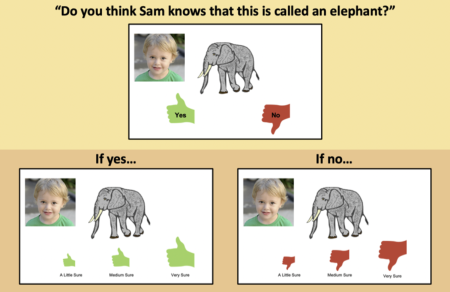
\includegraphics{figs/task-method-1} 

}

\caption[The general structure of an example trial]{The general structure of an example trial. The experimenter labels the animal, then asks the child “Do you think Sam knows that this is called an elephant?” Based on their response, children are then asked to provide a confidence judgment on a 3-point scale (little sure, medium sure, very sure).}\label{fig:task-method}
\end{figure}
\end{CodeChunk}

\emph{Introduction.} Children were shown a picture of a child named
``Sam'' (seen in Figure \ref{fig:task-method}). Children were anchored
to Sam's knowledge of various familiar skills, specifically some skills
that Sam has acquired (e.g., coloring), and some that Sam has not yet
acquired (e.g., reading). Children are then specifically anchored to
Sam's possible word knowledge in an unrelated domain-- given an example
of one whord Sam knows (\emph{car}), and one word that Sam doesn't know
(\emph{piano}). This introduction is intended to familiarize the
children with Sam, roughly anchor them to Sam's knowledge and age, and
to ensure that children understand there are things Sam doesn't know yet
(even things children themselves likely know, such as how to read).

\emph{General trial structure.} At each trial, children were shown a
drawing of a familiar object or animal (Rossion \& Pourtois, 2004). The
experimenter first labelled the object for the child (e.g., saying
``Look, it's {[}an elephant{]}!), and then asked the target child's
knowledge (e.g., saying,''Do you think Sam knows that this is called
{[}an elephant{]}? Yes or no?''). Based on their response, children are
then asked a follow-up question: ``How sure are you that Sam
{[}knows/doesn't know{]} that this is called {[}an elephant{]}-- a
little sure, medium sure, or very sure?'' All questions were presented
with accompanying pictures of thumbs {[}up/down{]} of varying size (see
Figure \ref{fig:task-method}). Children as young as 3 are able to engage
in uncertainty monitoring and report confidence, although these skills
do develop in the preschool years (Lyons \& Ghetti, 2011). Children's
responses to these two items were recoded onto a 1-6 scale from 1-very
sure Sam doesn't know to 6-very sure Sam knows. All trials followed this
general structure.

The experimenter provided no evaluative feedback on any trials, but did
offer consistent neutral feedback (e.g., repeating the child's answer or
saying ``Okay!''). When a child failed to respond within about 5 seconds
or offered a non-canonical response (e.g., saying ``Maybe''), the
experimenter acknowledged the child's answer and then repeated the
question with the possible responses. If a child did not answer after
the question was repeated, the experimenter moved on and marked the
trial as no response. These were considered ``incomplete'' sessions and
these participants were not included in the final sample.

\emph{Familiarization trials.} Children first completed two non-animal
familiarization trials, one of an early-acquired word (ball) and one of
a late-acquired word (artichoke). These trials followed the trial
structure described above and were intended to help familiarize children
with the structure of the questions and scales. These trials were always
asked first and in a fixed order.

\emph{Animal trials.} Children were then shown 15 trials of the same
form (see example trial in Figure \ref{fig:task-method}). For the 15
animal trials, trial order was randomized across participants to control
for any potential order effects in children's responses.

\emph{Explanation.} After completing the final animal trial, children
were asked an open-ended explanation question about their final
judgement (e.g., ``Why do you think Sam {[}knows/doesn't know{]} that
this is called {[}an elephant{]}?''). Because the trial order was
randomized, the explanations concerned different animal words across
participants.

\emph{Final check questions.} Children were asked two questions about
Sam's skill knowledge, one early acquired skill (going up and down
stairs) and one very late acquired skill (driving a car). These
questions again followed the general trial structure described above.
The skill knowledge items were included as an additional check that
children at all ages were able to use the scale appropriately, in case
young children failed to differentiate animal words based on AoA.
Lastly, children were asked to report how old they thought Sam was. This
question was intended to assess another aspect of children's belief
about Sam. Sam's photo and skill knowledge were intended to indicate
toddlerhood.

\hypertarget{adult-procedure.}{%
\paragraph{Adult procedure.}\label{adult-procedure.}}

Adult participants completed a minimally adapted version of the same
task online via Qualtrics. Unlike children, adults were simply presented
with the full 6-point scale (1 - \emph{very sure Sam doesn't know} to 6
- \emph{very sure Sam does know}). Additionally, the task was
administered asychronously, so adult participants did not interact with
an experimenter or recieve any feedback during the task. Otherwise, the
adult task was identical to the child task descirbed above.

\begin{CodeChunk}
\begin{figure}[tb]
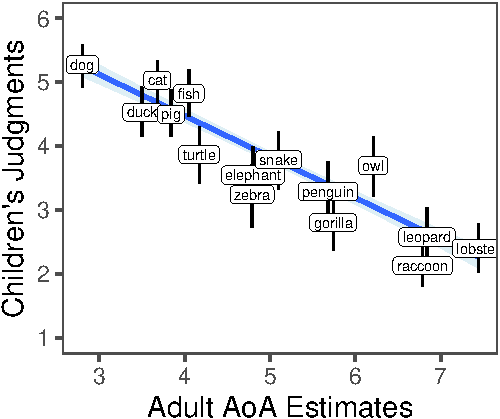
\includegraphics{figs/overall-1} \caption[Comparing adult AoA estimates (in years, taken from Kuperman et al., 2012) and children’s judgments on our 6-point scale (1 = very sure Sam doesn’t know]{Comparing adult AoA estimates (in years, taken from Kuperman et al., 2012) and children’s judgments on our 6-point scale (1 = very sure Sam doesn’t know; 6 = very sure Sam knows). The black lines show 95\% confidence intervals for each item. The shaded region shows one standard deviation based on a linear regression estimated from the raw data.}\label{fig:overall}
\end{figure}
\end{CodeChunk}

\hypertarget{results}{%
\section{Results}\label{results}}

Our primary analyses compare knowledge judgments on our 6-point scale to
AoA judgements from adults (taken from Kuperman et al., 2012). Data were
analyzed using pre-registered mixed effects model predicting children's
judgments from adult AoA estimates (Kuperman et al., 2012), including
random effects for participant and word. Using the lme4 package in R
(Bates, Mächler, Bolker, \& Walker, 2015), our model syntax was
\texttt{judgment\ \textasciitilde{}\ aoa\ +\ (1\ \textbar{}\ participant)\ +\ (1\textbar{}word)}.

We expected that overall, children's judgments would recover the ordinal
shape of age of acquisition data for these items. That is, children
would infer that the child is most likely to know early acquired words,
and least likely to know late acquired words. As a result, we expected a
negative relationship between judgments of the target child's lexical
knowledge and adult AoA estimates.

First, analyzing adults responses on our task, we see the predicted
negative effect of AoA on adult's judgements of the target child's
knowledge (see Figure \ref{fig:development}), \(\beta =\) -0.63, \(t =\)
-8.71, \(p\) \textless{} .01). This provides a simple sanity check that
our task is eliciting reliable predictions from adults, and that adults'
inferences about the target child's knowledge match predictions from AoA
estimation tasks (e.g., Kuperman et al., 2012).

\begin{CodeChunk}
\begin{figure*}[tb]
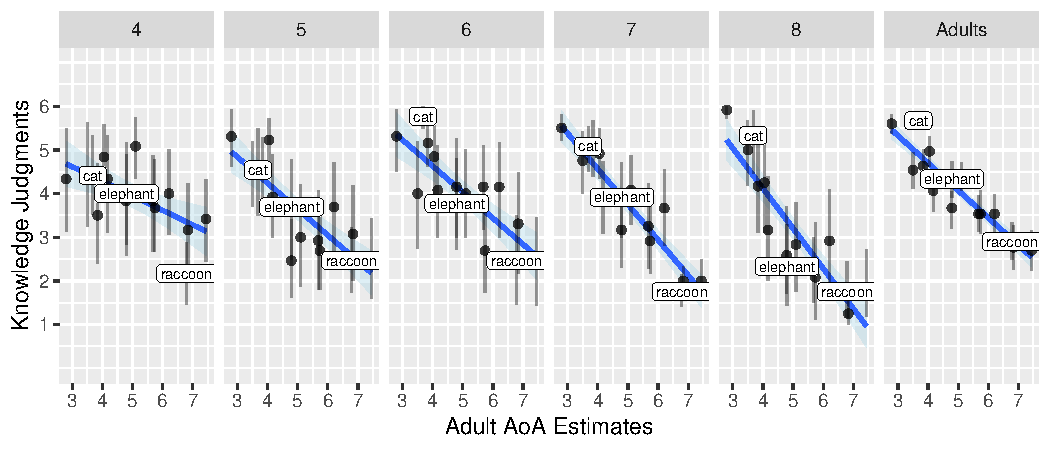
\includegraphics{figs/development-1} \caption[Children and adults judgements about the target child's word knowledge across development, compared with adult AoA estimates (in years, taken from Kuperman et al., 2012)]{Children and adults judgements about the target child's word knowledge across development, compared with adult AoA estimates (in years, taken from Kuperman et al., 2012). Each point represents 1 of the 15 word items, with black lines showing 95\% percent confidence intervals for each item. The shaded region shows one standard deviation based on a linear regression estimated from the raw data.}\label{fig:development}
\end{figure*}
\end{CodeChunk}

Do children's judgments about a child's vocabulary knowledge also
reflect a sensitivity to which words are learned later? To answer this
quetion looking at children's responses overall, we ran the model with
no age term and see a significant negative effect of AoA on children's
judgements (\(\beta =\) -0.65, \(t =\) -8.29, \(p\) \textless{} .001).
That is, overall, children judged that the target child would be most
likely to know an early acquired word (e.g., dog) and least likely to
know a late acquired word (e.g., lobster, see (Figure
\ref{fig:overall})).

We also expected developmental change in children's sensitivity to Sam's
vocabulary knowledge, with older children's judgments recovering
word-level AoA data more closely. To test for developmental changes in
children's responses, we used the same mixed effects model but included
an effect of age and an interaction between AoA and age. Our model
syntax was
\texttt{judgment\ \textasciitilde{}\ aoa\ *\ age\ +\ (1\ \textbar{}\ participant)\ +\ (1\textbar{}word)}.
We expected a significant interaction between AoA and child's age,
consistent with older children's judgments more closely reflecting
word-level AoA data. That is, when plotting children's judgments against
adult AoA estimates, older children would show steeper negative slopes
than younger children (Figure \ref{fig:development}). As above, our
model shows the same main effect of aoa that we saw in the overall model
(\(\beta =\) -0.65, \(t =\) -8.29, \(p\) \textless{} .001). We also see
a positive main effect of children's age on their ratings (\(\beta =\)
0.55, \(t =\) 3.68, \(p\) \textless{} .001). Crucially, we see our
expected interaction between child's age and adult's estimated AoA
(\(\beta =\) -0.14, \(t =\) -5.1, \(p\) \textless{} .001), suggesting
that children's judgements are becoming more adult-like in this age
range (Figure \ref{fig:development}).

To test the robustness of this intuition at each age, we ran the above
model separately for each year-wise age group. While we see evidence of
developmental change above, this additional analysis helps us understand
if even young children are showing this intuition. We found a
significant negative effect of AoA on children's judgments at all age
groups (with the smallest effect in 4-year-olds: \(\beta =\) -0.33,
\(t =\) -3.01, \(p =\) .01). That is, even 4-year-old children judged
that late-acquired animal words were less likely to be known by the
target child.

{[}\textbf{add results in brief about non-target questions, e.g., skills
knowledge}{]}

\hypertarget{explanations}{%
\subsubsection{Explanations}\label{explanations}}

As a secondary analysis, we were also interested in the reasons young
children gave for why the target child would or would not know a given
word. While children sometimes offered spontaneous explanations
throughout the study, this analysis focuses on the explanation elicited
after the final animal trial. Based on preliminary discussions between
the authors, the explanations were divided into 6 non-mutually-exclusive
categories: \emph{Language}, \emph{Experience}, \emph{Location},
\emph{Age}, \emph{Unsure}, and \emph{Other}.

\emph{Language} reflects explanations that explicitly appealed to
language properties. \emph{Experience} reflects explanations that appeal
to the child's real-world experience with the referent. \emph{Location}
reflects explanations that specifically reference a particular place the
animal is associated with. \emph{Age} reflects explanations that
reference a particular age or general age-group. Any child that failed
to answer the explanation question or expressed ignorance was coded as
giving an explanation of \emph{Unsure}. An explanation that didn't fall
into any of the above category was coded as \emph{Other}. Note that
coding was not mutually-exclusive, so explanations could be coded as
including multiple categories. See Table \ref{tab:explanations_table}
for examples of each coding category.

\begin{CodeChunk}
\begin{figure}[tb]
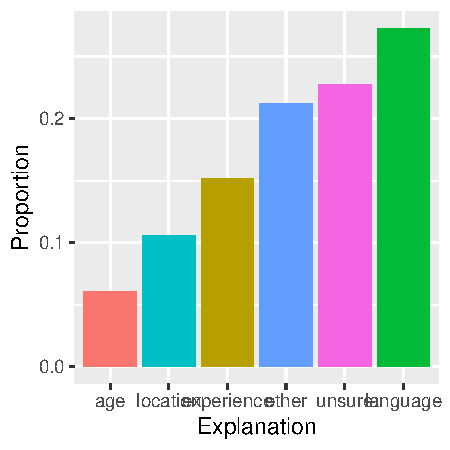
\includegraphics{figs/explanations-1} \caption[Children's explanations for why they think Sam knew/didn't know an animal]{Children's explanations for why they think Sam knew/didn't know an animal. Categories are not mutually exclusive.}\label{fig:explanations}
\end{figure}
\end{CodeChunk}

{[}\textbf{add explanation descriptives,} and by age{]}

Of the 6 types of explanations, \emph{Language} was used by the highest
proportion of children (27.27\%). \emph{Unsure} and \emph{Other}
explanations contributed to just under half of all the explanations
(22.73\% and 21.21\% respectively). Of the remaining three types,
children appealed to \emph{Experience} the most (15.15\%), followed by
\emph{Location} (15.15\%) and \emph{Age} (6.06\%; see Figure
\ref{fig:explanations}). Because coding categories were not mutually
exclusive, the proportions do not add to 1. To understand how children's
explanations may change over development, we median-split the data into
older and younger children. We find that older child {[}\textbf{what
older kids did}{]}, and younger children {[}\textbf{what younger kids
did}{]}.

\begin{table*}[tb]
\centering
\begin{tabular}{ll}
  \hline
Category & Example Utterance \\ 
  \hline
Language & Because it was a very long word. \\ 
  Experience & Because maybe he has a dog. \\ 
  Location & Because penguins live in the artic and it's too cold for little kids so that's why you should have 130 jackets... \\ 
  Age & Because I think I knew that when I was around 3, I knew what a pig was. \\ 
  Unsure & I don't know. \\ 
  Other & Because it had a longer beak than a bird. \\ 
   \hline
\end{tabular}
\caption{Example explanations from child participants for each of the five categories used for coding.} 
\label{tab:explanations_table}
\end{table*}

\hypertarget{discussion}{%
\section{Discussion}\label{discussion}}

Our ability to infer other people's knowledge is crucial for successful
communication. Young children are capable of inferring others' general
knowledge states, but do they make accurate judgments about another
person's specific knowledge? We asked 4- to 8-year-old children to
estimate another child's knowledge of animal words, and found that
children as young as 4 are sensitive to a younger child's lexical
knowledge. Children across age groups made judgments similar to those of
adults, with older children recovering more adult-like patterns.

Our findings indicate that young children have surprising metalinguistic
knowledge, and can use that knowledge to make highly-specific inferences
about other people's knowledge. The animal words used in our study are
generally learned within a 6-month period, yet young children could
still distinguish early-acquired words from late-acquired words in this
set. Our study also builds upon the extant literature on children's
inferences about other people's knowledge to show that children infer
others' specific, lexical knowledge. When given fairly minimal
information about another child, children readily make estimates about
that child's lexical knowledge.

How are children in our study making estimates about other people's
knowledge? One limitation of the current study is that it leaves the
mechanisms underlying such estimates unclear. Children's own
explanations suggest that they use various cues to make their estimates,
mostly appealing to {[}age/language/experience?{]}. {[}\textbf{adult
work?}{]}. Future should could more directly probe the features
underlying this inference-- to see if children are relying on their own
uncertainty, word length (and other linguistic cues), features of the
referent itself, or still other features.

The current work lays the foundation for future research on how children
leverage their knowledge of other people to communicate successfully.
Young children struggle in a variety of communicative tasks (e.g. Krauss
\& Glucksberg, 1977), and the current work can begin to map out whether
such difficulties stem from tracking an interlocutor's knowledge, or may
stem from problems using that information to adjust language production.
By at least age 5, children selectively talk about general or specific
characteristics of an object based on their partners' knowledge state,
when the knowledge state is salient and explicit for each item (Baer \&
Friedman, 2018). Based on our findings that children can reason about
others' specific knowledge, we can ask whether children's adaptations
extend to the level of lexical knowledge-- Do children adjust the way
they talk about a referent based on their beliefs about a partners'
knowledge of that word?

\vspace{1em} \fbox{\parbox[b][][c]{7.3cm}{\centering Stimuli, data, and analysis code available after deanonymization.}}

\hypertarget{references}{%
\section{References}\label{references}}

\setlength{\parindent}{-0.1in} 
\setlength{\leftskip}{0.125in}

\noindent

\hypertarget{refs}{}
\leavevmode\hypertarget{ref-baer2018}{}%
Baer, C., \& Friedman, O. (2018). Fitting the message to the listener:
Children selectively mention general and specific facts. \emph{Child
Development}, \emph{89}(2), 461--475.

\leavevmode\hypertarget{ref-bates2015}{}%
Bates, D., Mächler, M., Bolker, B., \& Walker, S. (2015). Fitting linear
mixed-effects models using lme4. \emph{Journal of Statistical Software},
\emph{67}(1), 1--48. \url{http://doi.org/10.18637/jss.v067.i01}

\leavevmode\hypertarget{ref-cycowicz1997}{}%
Cycowicz, Y. M., Friedman, D., Rothstein, M., \& Snodgrass, J. G.
(1997). Picture naming by young children: Norms for name agreement,
familiarity, and visual complexity. \emph{Journal of Experimental Child
Psychology}, \emph{65}(2), 171--237.

\leavevmode\hypertarget{ref-frank2017}{}%
Frank, M. C., Braginsky, M., Yurovsky, D., \& Marchman, V. A. (2017).
Wordbank: An open repository for developmental vocabulary data.
\emph{Journal of Child Language}, \emph{44}(3), 677--694.

\leavevmode\hypertarget{ref-krauss1977}{}%
Krauss, R. M., \& Glucksberg, S. (1977). Social and nonsocial speech.
\emph{Scientific American}, \emph{236}(2), 100--105.

\leavevmode\hypertarget{ref-kuperman2012}{}%
Kuperman, V., Stadthagen-Gonzalez, H., \& Brysbaert, M. (2012).
Age-of-acquisition ratings for 30,000 english words. \emph{Behavior
Research Methods}, \emph{44}(4), 978--990.

\leavevmode\hypertarget{ref-rossion2004}{}%
Rossion, B., \& Pourtois, G. (2004). Revisiting Snodgrass and
Vanderwart's object pictorial set: The role of surface detail in
basic-level object recognition. \emph{Perception}, \emph{33}, 217--236.

\leavevmode\hypertarget{ref-snodgrass1980}{}%
Snodgrass, J. G., \& Vanderwart, M. (1980). A standardized set of 260
pictures: Norms for name agreement, image agreement, familiarity, and
visual complexity. \emph{Journal of Experimental Psychology: Human
Learning and Memory}, \emph{6}(2), 174.

\leavevmode\hypertarget{ref-walley1992}{}%
Walley, A. C., \& Metsala, J. L. (1992). Young children's
age-of-acquisition estimates for spoken words. \emph{Memory \&
Cognition}, \emph{20}(2), 171--182.

\bibliographystyle{apacite}


\end{document}
